
\documentclass[12pt]{article}
\usepackage{geometry} % see geometry.pdf on how to lay out the page. There's lots.
\usepackage{subfig}
\usepackage{parskip}
\usepackage{graphicx}


\geometry{letterpaper} % or letter or a5paper or ... etc
% \geometry{landscape} % rotated page geometry

% See the ``Article customise'' template for come common customisations

\title{Final Report}
\author{}
%\date{} % delete this line to display the current date

%%% BEGIN DOCUMENT
\begin{document}

\maketitle

%%%%%%%%%%%%%%%%%%%%%%%%%%%%%%%%%%%%%%%%%%%%%%%%
% Section 1
%%%%%%%%%%%%%%%%%%%%%%%%%%%%%%%%%%%%%%%%%%%%%%%%
\section{Introduction}
Recommender System is becoming a crucial part of our online experience these days. It is widely used in various websites to recommend all kinds of products to customers: movies\footnote[1]{www.flixster.com}, books\footnote[2]{www.amazon.com}, music\footnote[3]{www.pandora.com}, etc. The quality of a recommender system is not only related to user experience, but also revenues of online business.  

Different recommendation methods have been proposed in both industry and academia. The performance of recommender systems is usually measured with two metrics: accuracy and coverage. Higher accuracy means the estimated rating of one item for target user is more likely to match the user's own rating of that item; higher coverage means the system is able to predict more items' ratings for more users. 

One of the most popular recommendation method is Collaborative Filtering (CF) \cite{Sarwar:2001p125}. CF compares rating profiles of all items and identifies \emph{similar items} using Pearson Correlation. When asked to predict the rating of a target item for a target user, CF first finds items which are similar to the target item, then it returns the target user's average ratings of these similar items (weighted by their similarities to the target item). Though CF has been adopted by many recommender systems, it performs poorly for cold-start users (i.e. new users of a website). Since cold-start users have rated only a few items, it is often difficult for CF to find similar items rated by the target user. Therefore, coverage of CF is usually very low for cold-start users. 

To overcome the weakness of CF on cold-start users, Mohsen Jamali and Martin Ester proposed Trustwalker \cite{Jamali:2009p67}. Trustwalker combines trust-based method and CF by performing a random walk on the target user's neighbours (both direct and indirect). Trustwalker managed to achieve lower Root Mean Square Error (RMSE) and higher coverage compared to traditional CF. 

To explore potential improvement in these recommender systems mentioned above, we propose a new recommendation method, which utilizes users' expertise in different product categories. The rationale behind this method is that experts' reviews tend to be more insightful and cover more items. Besides, according to consumer psychology, consumers tend to trust more on experts when they are purchasing more expensive products, such as cars, electronics, etc \cite{consumer}. We first calculate all users' expertise based on the number and qualities of their reviews, then we pick users with the highest expertise and call them \emph{experts}. Lastly, we use experts' ratings to predict the ratings of other users. 

The rest of the report is organized as follows: section 2 introduces the methodology of our experiments; section 3 reports the dataset we crawled from Epinions.com and our experiment results on that dataset; section 4 concludes the project. 

%%%%%%%%%%%%%%%%%%%%%%%%%%%%%%%%%%%%%%%%%%%%%%%%
% Section 2
%%%%%%%%%%%%%%%%%%%%%%%%%%%%%%%%%%%%%%%%%%%%%%%%
\section{Methodology}
This section introduces the key steps in the project. 

\subsection{Identifying Experts} % (fold)
\label{sub:identifying_experts}

Given a category $C$ and a set of users $U = \{{u_{1}, ..., u_{n}}\}$ who have written at least one review in category $C$, we primarily consider two factors in calculating a user's expertise: (1) the average quality of the user's reviews, and (2) the total number of user's reviews. We use the following formulas to calculate a user's expertise in a category $C$:
\begin{equation}
E(u) = \frac{\sum_{i=1}^n R_{u, i}} {n} \times f(n)
\end{equation}
\begin{equation}
f(n) = \frac{1}{1 + e^{\frac{-10n} {MAX\_REVIEWS(C)}}}
\end{equation}
where $R_{u, i}$ is the rating for user $u$'s review $i$ in category $C$ and $f(n)$ is a sigmoid function to avoid favoring the number of reviews too much. It is based on the assumption that a user written 100 reviews has more expertise than a user written 10 while a user written 1000 reviews is almost as good as a user written 900 reviews. $MAX\_REVIEWS(C)$ is the maximum number of reviews per user in category $C$. $f(n)$ is tailored for every category, i.e., the user who has written the most reviews in a category have $f(n)=1$.

% subsection identifying_experts (end)

\subsection{Top $k$ Experts Recommendation} % (fold)
\label{sub:expert_recommendation}

Previous research has demonstrated that recommending items to users based on \emph{expert} opinions can be as good as traditional user-based \emph{Collaborative Filtering} \cite{Amatriain:2009p101}. We propose a similar expert recommendation algorithm: given an item $i$ that belongs to a category $C$, the recommender first picks out the top $k$ percent experts in category $C$; then for each expert, if the expert has rated item $i$, the exact rating is returned; otherwise a weighted average of similar items of $i$ is returned; finally the recommender averages the ratings of all selected experts by their expertise as the predicted rating for item $i$. 

Item similarity is calculated using \emph{Pearson Correlation}:
\begin{equation}
	corr(i,j) = \frac{\sum_{u \in U_{i,j}} (r_{u,i} - \bar{r}_u)(r_{u,j} - \bar{r}_u)} {{\sqrt{\sum_{u \in U_{i,j}} (r_{u,i} - \bar{r}_u)}} \sqrt{\sum_{u \in U_{i,j}} (r_{u,j} - \bar{r}_u)}}
\end{equation}
where $U_{i,j}$ is the set of common users who have rated both items $i$ and $j$, and $\bar{r}_u$ denotes the average of ratings expressed by $u$. Pearson correlation $corr(i,j)$ is in the range $[-1,1]$. Negative correlation means that two items are correlated. Thus we only consider positive correlation.

When predicting the item $i$'s rating for user $u$, the recommender consults the opinions from the set of experts $E = \{e_1, e_2, ...\}$. If expert $e$ has rated item $i$, the prediction is calculated directly as:
\begin{equation}
	\hat{r}_{e,i} = \bar{r}_u + (r_{e,i} - \bar{r}_e)
\end{equation}
where $\bar{r}_u$ is the average rating of user $u$ and $\bar{r}_e$ is the average rating of expert $e$. If expert $e$ has not rated the item $i$, the prediction is calculated using weighted average of similar items rated by the expert:
\begin{equation}
	\hat{r}_{e,i} = \bar{r}_u + \frac{\sum_{j \in I_{sim}} (r_{e,j} - \bar{r}_e) \times corr(i,j)} {\sum_{j \in I_{sim}} corr(i,j)}
\end{equation}
where $I_{sim}$ is the item set similar to item $i$. The recommender aggregates all the experts opinions as the final prediction for user $u$:
\begin{equation}
	\hat{r}_{u,i} = \frac{ \sum_{e \in E} \hat{r}_{e,i} \times exp(e) } { \sum_{e \in E} exp(e) }
\end{equation}
where $exp(e)$ is the expertise of expert $e$.

We also implemented a simple version of top $k$ experts recommendation. In this version, when predicting a rating of item $i$ for user $u$, the recommender only consults experts who have rated item $i$. Experts who have only rated similar items of $i$ are not consulted.
 
% subsection expert_recommendation (end)



%%%%%%%%%%%%%%%%%%%%%%%%%%%%%%%%%%%%%%%%%%%%%%%%
% Section 3
%%%%%%%%%%%%%%%%%%%%%%%%%%%%%%%%%%%%%%%%%%%%%%%%
\section{Experiment}
We tested different recommender systems on a comprehensive dataset from Epinions.com, which is a product reviewing site for consumers. This section reports our findings in the experiments.  
\subsection{Dataset}
Epinions.com is a website where users can rate products and write reviews. Its product catalogue covers a large number of product categories, including Music, Books, Movies, Automobiles, Electronics, etc. For each product, consumers provide ratings on a scale from 1 to 5 (5 being the best), write detailed reviews on products and express the helpfulness of existing reviews. Besides, users can express directed trust among each other: if user A trusts user B, user B does not have to trust user A. In other words, there is a implicit directed trust graph among all users. 

We crawled a comprehensive dataset from Epinions.com, which includes user info, product reviews, review helpfulness, trust links, etc. The size of the crawled dataset is shown in Table ~\ref{data_size}. Among all the 91,584 users, about 1000 users have written more than 100 reviews. These top 1000 most productive users have contributed to 55.9\% reviews (338,173 out of 605,066).  Table ~\ref{rating_distro} shows the distribution of ratings among all products. One third of the ratings are 5, and about 60\% of the ratings are 4 or 5. The distribution is very different from another popular dataset -- MovieLens, whose rating distribution is more diverse\footnote[1]{http://www.grouplens.org/node/73}. Table ~\ref{helpful_distro} shows the helpfulnesses of all reviews. Similarly, about 75\% of all reviews are considered \emph{very helpful}. 

Table ~\ref{category_distro} shows the number of reviews in the top 5 categories. The top 5 categories account for more than half of all reviews on Epinions.com.

\begin{table}
	\centering
	\subfloat[Dataset Size\label{data_size}] {
		\begin{tabular}[b] {| l | r | }
			\hline
			Data Type & Size \\ \hline \hline
			Users & 91,584 \\ \hline
			Reviews & 605,066 \\ \hline
			Trust Links & 1,152,095 \\
			\hline
		\end{tabular}
	}	
	\subfloat[Rating Distribution\label{rating_distro}] {	
		\begin{tabular}[b] {| c | r |}
		\hline
		Rating & Percentage \\ \hline \hline
		5 & 33\% \\ \hline
		4 & 27\% \\ \hline
		3 & 20\% \\ \hline
		2 & 13\% \\ \hline
		1 & 7\% \\
		\hline
		\end{tabular}
	}
	\subfloat[Review Helpfulness Distribution \label{helpful_distro}] {		
		\begin{tabular}[b] {| l | r | }
		\hline
		Review Helpfulness & Percentage \\ \hline \hline
		Very Helpful & 74.3\% \\ \hline
		Helpful & 15.4\% \\ \hline
		Somewhat Helpful & 6.8\% \\ \hline
		Show & 2.4\% \\ \hline
		Not Yet Rated & 1\% \\
		\hline
		\end{tabular}
	}

	\caption{Dataset Summary}
\end{table}

\begin{table}[h]
	\centering
	\begin{tabular} {| l | c | r | }
		\hline
		Category & Number of Reviews & Percentage \\ \hline \hline
		Movies & 102,461 & 16.9\% \\ \hline
		Books & 72,940 & 12.1\% \\ \hline
		Music & 63,424 & 10.5\% \\ \hline
		Hotels \& Travel & 32,348 & 5.3\% \\ \hline
		Electronics & 31,853 & 5.3\% \\
		\hline
	\end{tabular}
	\caption{Product Categories of Reviews}
	\label{category_distro}
\end{table}

To test the performance of recommender systems, we split the dataset into a training set and a testing set. Testing set is chosen randomly from all ratings and takes about 20\% of all ratings; training set is the rest, which is about 80\%. Then we used the training set to predict the ratings in the testing set. To make the prediction more challenging, we pick out the ratings for controversial items from the testing set and measure the performance separately for these items. We define \emph{controversial items} to be the items whose ratings' Standard Deviations are greater than 1.5. These items' ratings are harder to predict, because users' opinions towards these items varies wildly from 1 to 5. The reason why we set a separate testing set for controversial items is that the ratings on Epinions.com are cluster around 4 and 5. Therefore, performing another experiment on controversial items could bring more insight on how the nature of this dataset affects the recommendation methods' performance. 

We used two most adopted metrics to measure the performance of recommender systems: Root Mean Square Error (RMSE) and coverage. In addition, we combined \emph{RMSE} and \emph{coverage} into a single metric called \emph{F Measure} \cite{Jamali:2009p67}. We define \emph{precision} and \emph{F Measure} similarly:
\begin{equation}
Precision = 1 - \frac{RMSE}{4}
\end{equation}

\begin{equation}
F Measure = \frac{2 \times Precision \times Coverage}{Precision + Coverage}
\end{equation}

The next subsection reports the performance of different recommender systems in the Epinions.com dataset. 

\subsection{Experimental Results}
Besides two \emph{Top-k expert} methods, we also implemented item-based CF and Trustwalker to compare the performance. The four methods in our experiments are:

\begin{enumerate}
	\item \emph{itemCF}. This is the traditional CF method, which returns the weighted average ratings of similar items from target user's rating profile. 
	\item \emph{Trustwalker}. This is the random walk model proposed by Mohsen Jamali and Martin Ester \cite{Jamali:2009p67}. We set the \emph{max\_depth} to 3 and \emph{epsilon} to 0.001 in their \emph{Trustwalker} model.
	\item \emph{expert}. This method finds the top-k experts in each category, then calculates weighted average of experts' ratings for target item and also similar items. The estimated rating is adjusted according to target user's rating scale. 
	\item \emph{expert-simple}. This is the simpler version of \emph{expert} method. It finds the top-k experts in each category, and returns the experts' weighted average ratings for the exact target item. The estimated rating is adjusted according to target user's rating scale. 
\end{enumerate}

We also implemented a version of Trustwalker which utilizes the expertise of each user, and return user's rating weighted by their expertise. However, this method performs almost the same as the original Trustwalker. Thus, the results are not shown in this report. 

\begin{figure}[htbp]
	\centering
	\subfloat[RMSE for all users]{\label{rmse_all}
			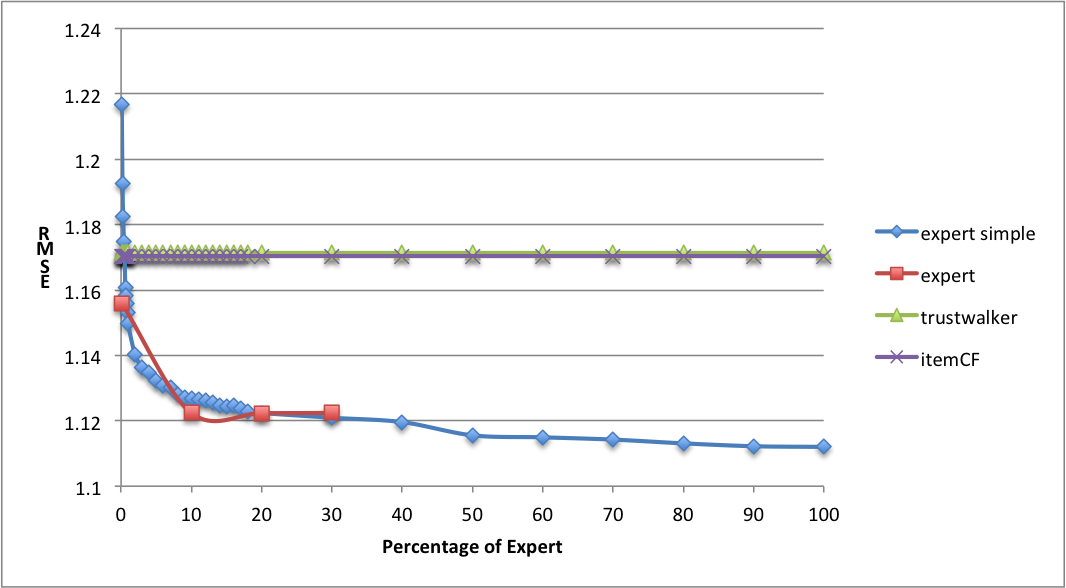
\includegraphics[width=12cm]{graphics/all_user_2.png}			
	}
	\\
	\subfloat[RMSE for cold-start users]{\label{rmse_cold}
			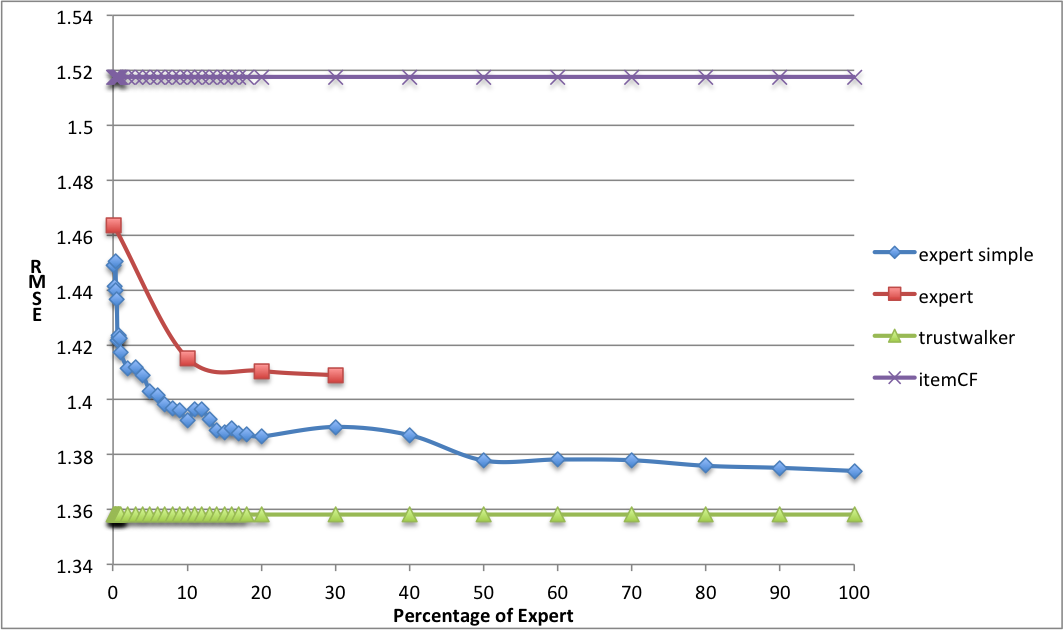
\includegraphics[width=12cm]{graphics/coldstart_user_2.png}			
	}
	\caption{RMSE}
\end{figure}

\begin{figure}[htbp]
	\centering
	\subfloat[Results for all users]{\label{results_all}
			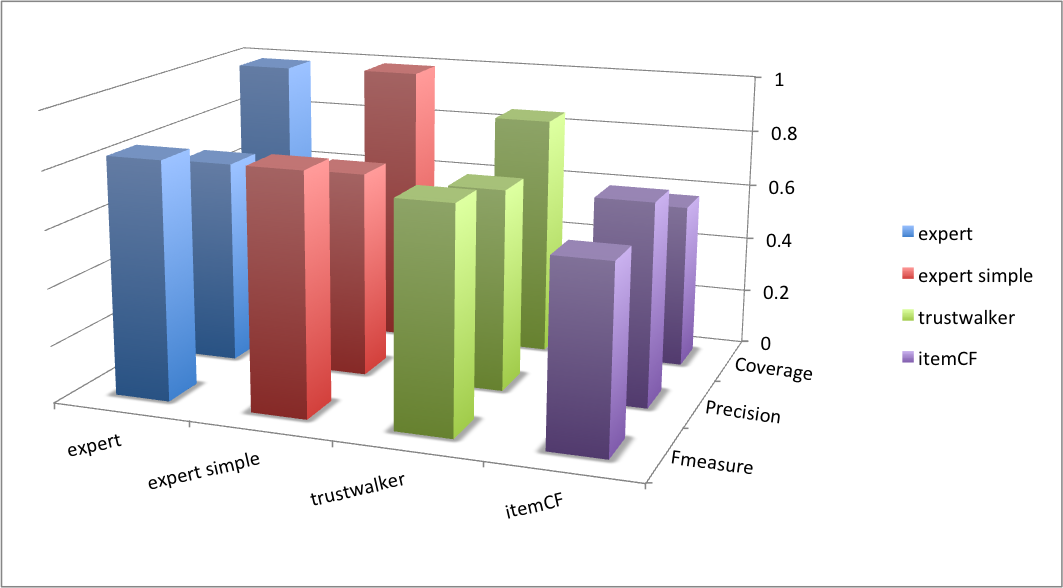
\includegraphics[width=12cm]{graphics/all_user.png}			
	}
	\\
	\subfloat[Results for cold-start users]{\label{results_cold}
			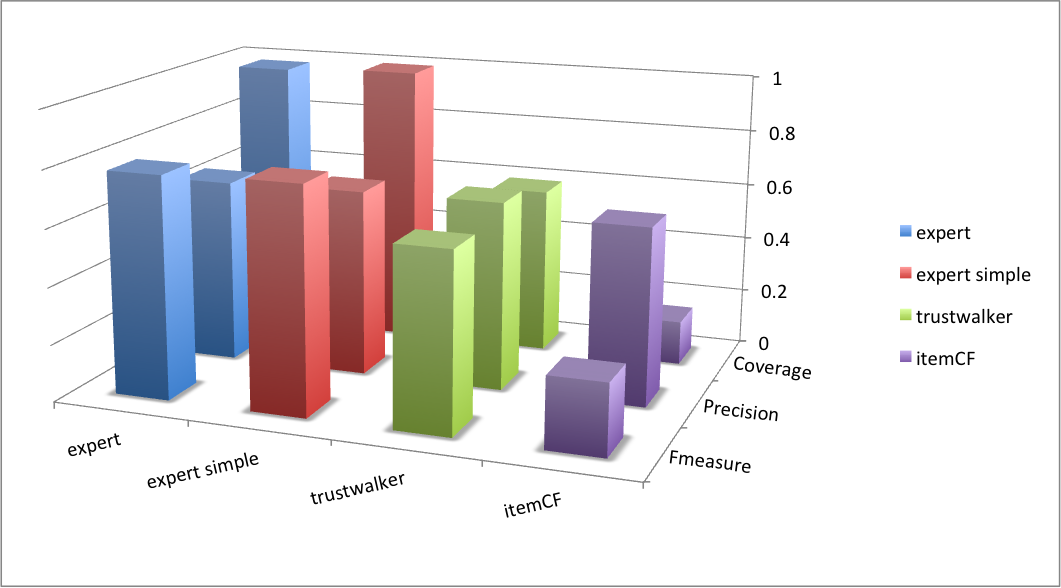
\includegraphics[width=12cm]{graphics/coldstart_user.png}			
	}
	\caption{Coverage, precision and F Measure}
\end{figure}

Figure ~\ref{rmse_all} and ~\ref{rmse_cold} shows the RMSE of the four methods over the entire testing set. The horizontal axis represents the percentage of users that we call experts. If the percentage is k\%, it means that we take the top k\% of users with the highest expertise in each category. Since y axis is only related to \emph{expert-simple} and \emph{expert} method, the performance of \emph{itemCF} and \emph{Trustwalker} remains the same. 

As shown in Figure ~\ref{rmse_all}, \emph{expert-simple} and \emph{expert} almost always perform better than \emph{itemCF} and \emph{Trustwalker}. This result is very surprising, since \emph{expert-simple} and \emph{expert} are relatively simple and naive methods compared to \emph{itemCF} and \emph{Trustwalker}. Besides, though the estimated ratings in \emph{expert-simple} and \emph{expert} are not personalized at all, the RMSE over all users are still quite good. 

Figure ~\ref{rmse_cold} shows the RMSE of the four methods over cold-start users in the testing set. For cold-start users, \emph{itemCF} performs poorly, since it could not find many ratings for similar items from the target user's rating profile. \emph{Trustwalker} performs better than both \emph{expert-simple} and \emph{expert}. This result is expected, since \emph{Trustwalker} was designed to mitigate the cold-start user's problem. 



Besides RMSE, the other most widely used metric in recommender system is coverage. We calculated the coverage, precision and F Measure of our experiment results. Precision and F Measure are discussed earlier in the previous section. Figure ~\ref{results_all} and ~\ref{results_cold} shows the precision, coverage and F measure of all four methods over all users and cold-start users. 

In Figure ~\ref{results_all}, F Measure of \emph{expert} and \emph{expert-simple} are higher than \emph{Trustwalker} and \emph{itemCF}, meaning that their overall performance is better than the latter two methods. The precisions of \emph{expert} and \emph{expert-simple} are similar to the precision of \emph{Trustwalker}. 

Figure ~\ref{results_cold} shows the performance of the four methods on cold-start users. The coverage of \emph{itemCF} is extremely low, which is less than 20\%. While \emph{Trustwalker} greatly improved the coverage compared to \emph{itemCF}, \emph{expert} and \emph{expert-simple} are much better in terms of coverage. Notice that the precision of \emph{Trustwalker} is the highest, though its F Measure is not as high due to its smaller coverage. If we compare F Measure, \emph{expert} and \emph{expert-simple} are still the two highest.

\begin{figure}[htbp]
\centering
	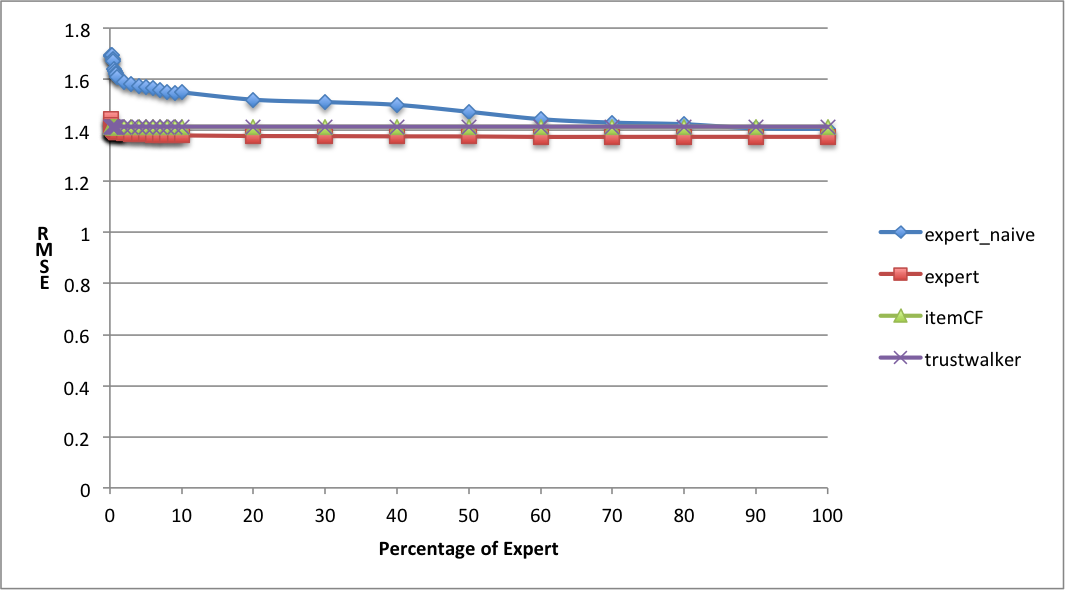
\includegraphics[width=12cm]{graphics/con_all_user.png}	
	\caption{RMSE of \emph{controversial items}}
	\label{con_all_user}
\end{figure}

Since the performance of non-personalized methods \emph{expert} and \emph{expert-simple} are surprisingly good up to now, we tested all four methods on a subset of our testing set, which only contains \emph{controversial items}. We have already defined controversial items in previous section to be the items whose ratings' Standard Deviations are greater than 1.5. We expect \emph{expert} and \emph{expert-simple} to perform worse in this dataset since they are non-personalized methods. Figure ~\ref{con_all_user} shows the RMSE of the estimated ratings for controversial items. The performance of two personalized methods \emph{itemCF} and \emph{Trustwalker} are similar to the two non-personalized methods \emph{expert} and \emph{expert-simple}. However, notice that the performance of \emph{expert} and \emph{expert-simple} has already decreased significantly. 

%%%%%%%%%%%%%%%%%%%%%%%%%%%%%%%%%%%%%%%%%%%%%%%%
% Section 4
%%%%%%%%%%%%%%%%%%%%%%%%%%%%%%%%%%%%%%%%%%%%%%%%
\section{Conclusion}
We calculated users' expertise using the number of qualities of their reviews. Then we pick users with highest expertise in each category and identify them as experts. We implemented two recommendation methods based on experts, and tested them against the dataset we crawled from Epinions.com. 

Initially we wanted to incorporate expertise of each user into Trustwalker and improve its accuracy. However, experiments show that this method is no better than original Trustwalker. On the other hand, more naive method \emph{expert} and \emph{expert-simple} perform surprisingly well in terms of both accuracy and coverage. This could be resulted from the nature of our dataset, where ratings are clustered around 4 and 5. 

Based on our experiment results, we argue that more complicated method may not be necessary in some scenarios. For example, if the reviewed products are more objective and less subjective, simply averaging experts' opinions could be comparable or better to trust-based method. For subjective products like music and movies, more complicated and personalized method usually out-performs naive averaging and are desired. 

\bibliographystyle{ieeetr}
\bibliography{references}


\end{document}